\newpage
\section{Versionsverwaltung Git}
Git ist eine freie Software zur verteilten Versionsverwaltung von Dateien, die urspr�nglich f�r die Quellcode-Verwaltung des Linux-Kernels entwickelt wurde. Git speichert die Daten nicht auf einen zentralen Server sondern bei jedem User zun�chst lokal in einem s.g. Repository. So besitzt jeder User den gesamten Code so wie die Versionsgeschichte zun�chst auf seinem eigenen PC. Ein Remote Repository ist ein Repository das nicht lokal auf dem eigenen Rechner verf�gbar ist sondern zentral auf einem Server ausgelagert wird. �ber einen Push Befehl kann das Remote Repository mit dem lokalem Repository �berschrieben werden. Wird ein Fetch Befehl ausgef�hrt wird dass Remote Repository mit dem lokalem Repository verglichen und zusammengef�hrt (merge Befehl) werden. Im Projekt wurde GitHub, ein webbasierter Hosting-Dienst f�r Software-Entwicklungsprojekte verwendet.


\begin{figure}[h]

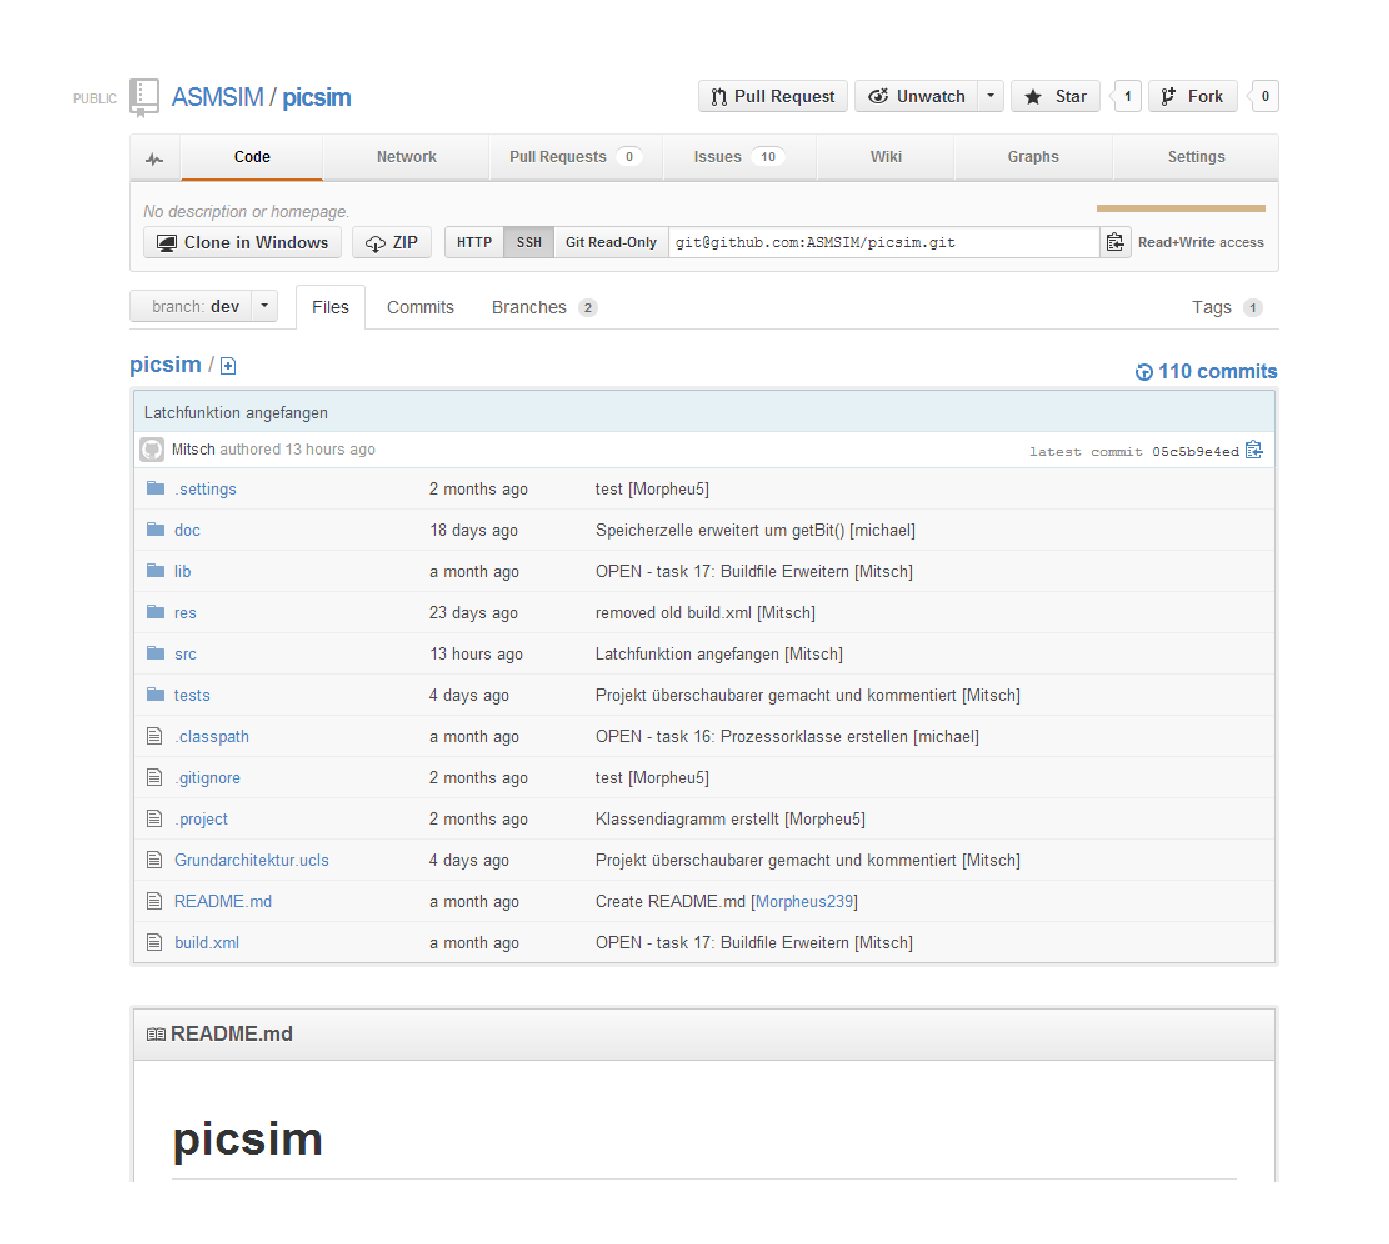
\includegraphics[scale=0.55]{Bilder/Github.pdf}
\caption{Github}
\end{figure}
